\documentclass{article}
\usepackage{times}
\usepackage{a4wide}
\usepackage{latexsym}
\usepackage{mathrsfs}
\usepackage{amsmath}
\usepackage{amssymb}
\usepackage{amsthm}
\usepackage{ifthen}
\usepackage{stmaryrd}
\usepackage{algorithm}
%\usepackage{algorithmic}
\usepackage{algpseudocode}
\usepackage{graphics}
\usepackage{epsfig}
\usepackage{graphicx}
\usepackage{subfigure}
%\usepackage{ramacros}

\addtolength{\textwidth}{20mm}
\addtolength{\oddsidemargin}{-10mm}
\addtolength{\textheight}{18mm}
\addtolength{\topmargin}{-9mm}

\newcounter{exercise}
\setcounter{exercise}{0}
\newcommand{\exercise}{
        \addtocounter{exercise}{1}
        \vspace{0.2in}
        \noindent
        {\bf \theexercise .}
        }

\newcommand{\REMARK}[1]{}


\newcommand{\NEWPART}{\vspace{.1in}
              \noindent}

\newcommand{\<}{
    \langle}

\renewcommand{\>}{
    \rangle}

\newcommand{\ceil}[1]{\left\lceil #1 \right\rceil}

\pagestyle{plain} \pagenumbering{arabic}

\title{{\bf Assignment 2} \\ {\large ID: 120037910002 } {\large Name: Xingguo Jia } {\large Email: jiaxg1998@sjtu.edu.cn}}


\author{}
\date{}

\begin{document}
\maketitle

%{\large \noindent
%\begin{tabular}{lcl}
%{Jan 17 2007}.
%\end{tabular}
%}

{\large





\begin{exercise}
\textsf{STINGY SAT} is the following problem: given a set of clauses(each a disjunction of literals) and an integer $k$, find a satisfying assignment in which at most 
$k$ variables are true, if such an assignment exists. Prove that \textsf{STINGY SAT} is NP-complete.
\end{exercise}
\begin{proof}
    \leavevmode\newline
    \begin{itemize}
        \item First we prove {STINGY SAT} is NP. Given an assignment, we can count the number of true variables. If the number is at most $k$, then such an assignment exist. This runs in  $O(l)$, where $l$ is the number of clauses. Thus, we can verify {STINGY SAT} in polynomial time, and it is NP.
        \item Then we reduce {SAT} to {STINGY SAT}. Given a set of $l$ clauses, once we find a satisfying assignment in which at most $k=l$ variables are true, then we solve the SAT problem. If we solve {STINGY SAT}, then we could solve {SAT} by setting $k$ to $l$. Since {SAT} is \textbf{NP} and the reduction takes polynomial time, {STINGY SAT} is \textbf{NP-complete}.
    \end{itemize}
\end{proof}
\newpage

\begin{exercise}
You are given a directed graph $G=(V,E)$ with weights we on its edges $e\in E$. The weights can be overlineative or positive. The \textsf{ZERO-WEIGHT-CYCLE PROBLEM} is to decide if there is a simple cycle in $G$ so that the sum of the edge weights on this cycle is exactly $0$. Prove that this problem is NP-complete.
\end{exercise}
\begin{proof}
    \leavevmode\newline
    \begin{itemize}
        \item The problem is NP since given a simple cycle in $G=(V,E)$, we can verify whether the sum of the edge weights on this cycle is exactly $0$ by adding all $|E|$ edge weights together, which costs $O(|E|)$ (polynomial) time.
        \item We reduce \textbf{subset-sum} problem to \textbf{zero-weight-cycle} problem, and since {subset-sum} problem is \textbf{NP}, zero-weight-cycle problem is \textbf{NP-complete}. For a set of number $a_i(i=1,\ldots ,n)$, decide whether there exists a subset whose sum is $0$.
        \item See Figure \ref{fig:ccc}, each vertex $u_i(i=1,\ldots ,n)$ has only one outgoing edge $u_i\rightarrow v_i$ with weight $a_i$, and each vertex $v_i(i=1,\ldots ,n)$ has $n$ outgoing edges to each $u_k(k=1,\ldots,n)$ with weight $0$. Any simple cycle in this graph has the form
        \item $u_{i_1}\rightarrow v_{j_1}\rightarrow u_{i_2}\rightarrow v_{j_2}\rightarrow \cdots \rightarrow u_{i_k}\rightarrow v_{j_k} \rightarrow u_{i_1}(1\leq k\leq n)$
        \item which has a weight sum of $\sum\limits_{j=1}^{k}a_{i_j}(1\leq k\leq n)$. This is a subset sum of set $\{a_i\mid i=1,\ldots ,n\}$. Thus, we could reduce the subset sum problem to zero-weight-cycle problem in $O(n)$ (polynomial) time.
    \end{itemize}
    \begin{figure}[!htp]
        \centering
        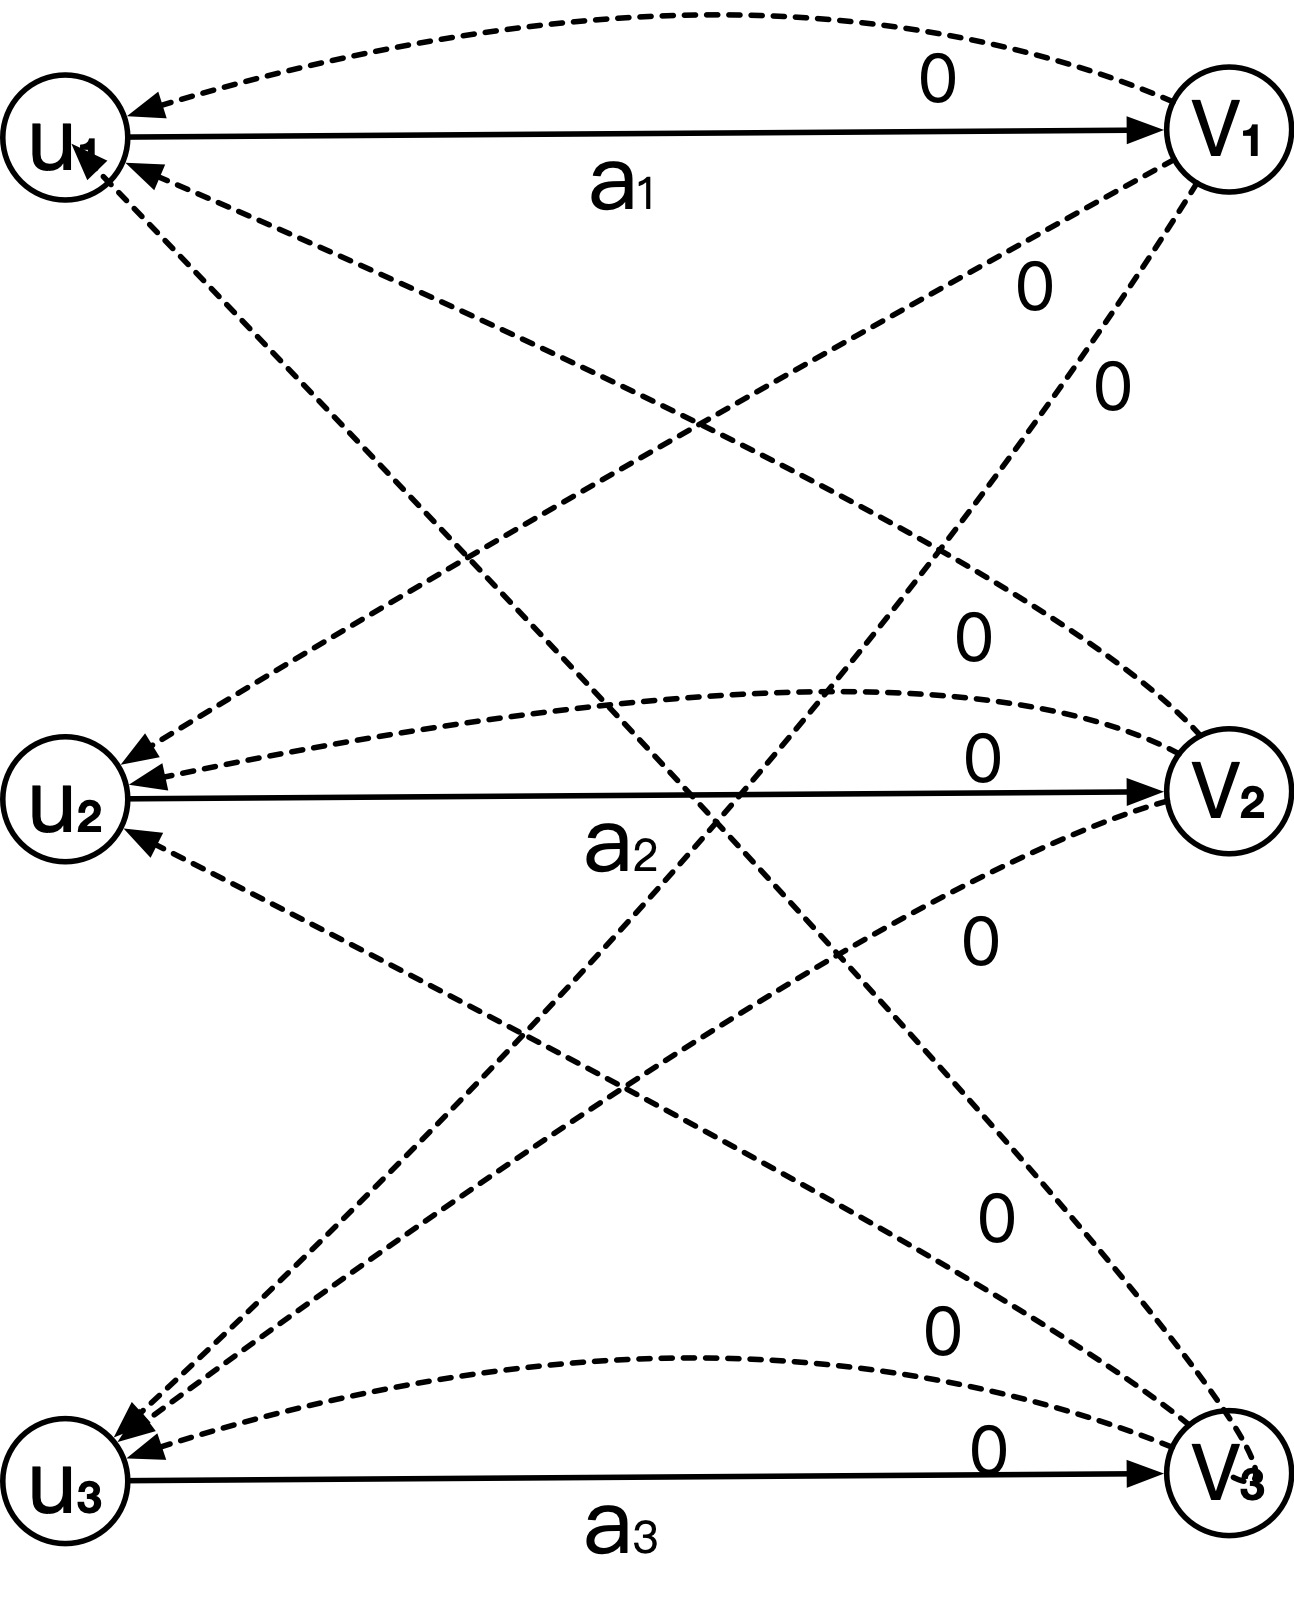
\includegraphics[width=0.35\textwidth]{img/4.jpg}
        \caption{Reduction from subset-sum problem}
        \label{fig:ccc}
      \end{figure}
\end{proof}
\newpage

\begin{exercise}
Show that \textsf{INDEPENDENT SET PROBLEM} is NP-hard even graphs of maximum degree $3$.
\end{exercise}
\begin{proof}
    \leavevmode\newline
    \begin{itemize}
        \item We reduce the \textbf{3-SAT} problem to \textbf{independent set} problem for a graph $G$ of maximum degree of $3$.
        \item For each clause in the formula, we use a vertex in $G$ to represent each literal of the clause, and add an edge between each of them. For each pair of opposite vertices between different clauses, add an edge between them. This reduction runs in $O(|V|+|E|)$ (polynomial) time.
        \item For example, Figure \ref{fig:eee} shows $G$ equivalent to formula ($-y$ stands for $\overline{y}$)
        \begin{displaymath}
            (x\vee y \vee z)(x \vee \overline{y})(y \vee \overline{z})(z \vee \overline{x})(\overline{x} \vee \overline{y} \vee \overline{z})
        \end{displaymath}
        \item For each clause $C_i(i=1,\ldots,n)$, we choose a $v_i$ in $G$. If all $v_i$ forms an independent set, then we set the literal to $true$ corresponding to $v_i$ and no opposite literals are set to $true$ at the same time. Thus we reduce \textbf{3-SAT} problem to \textbf{independent set} problem. 
        \begin{figure}[!htp]
            \centering
            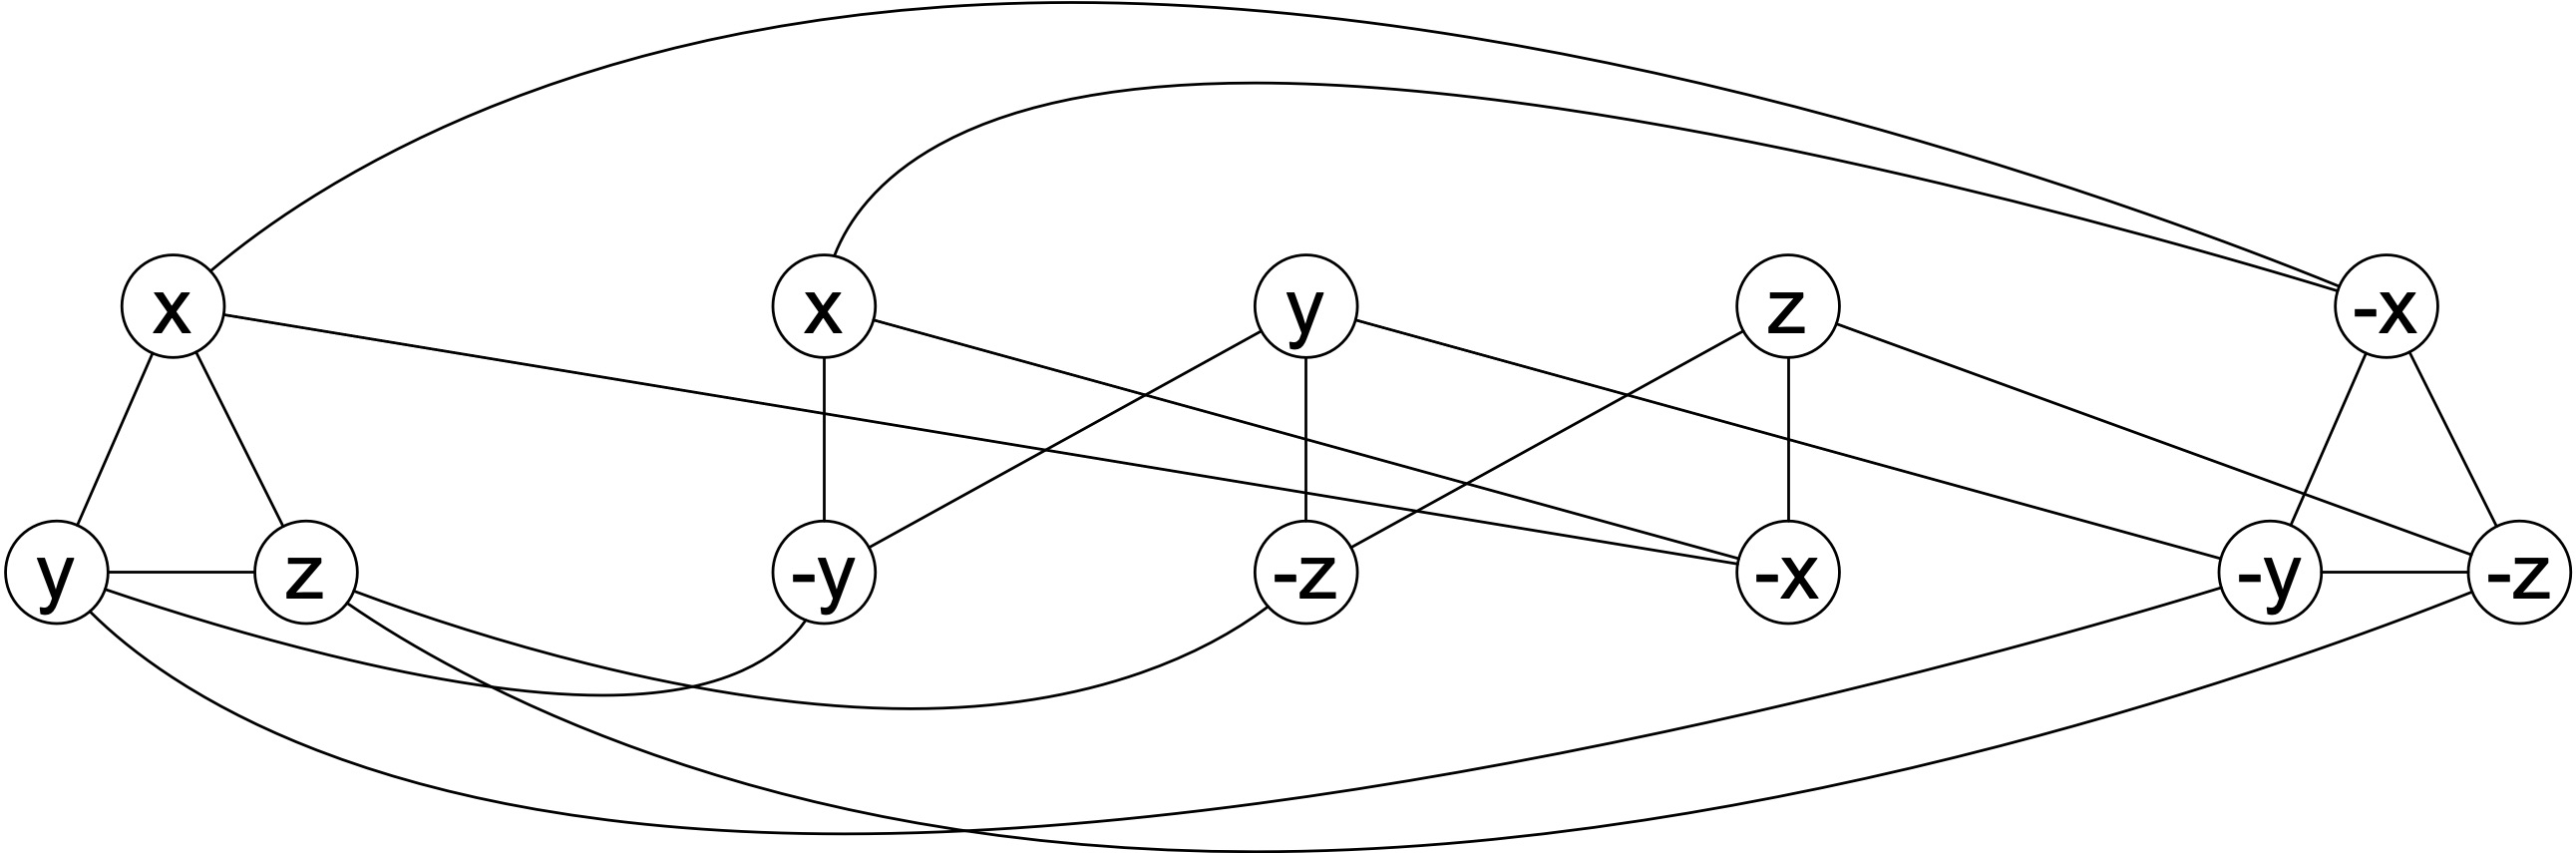
\includegraphics[width=0.7\textwidth]{img/5.jpg}
            \caption{Reduction from 3—SAT problem}
            \label{fig:eee}
          \end{figure}
        \item But in this graph, the maximum degree can be larger than $3$. We modify the formula to a \textbf{equivalent} one in the following way: if variable $x$ appears in $k\geq 3$ clauses, then in $G$, vertices corresponding to $x$ may have a degree $\geq 4$. For variable $x$ that appears in $k\geq 3$ clauses, modify the $k\ x$ variables to $x_1,x_2,\ldots,x_k$, and
        \begin{displaymath}
            F'=F\wedge U,U=(x_1\vee \overline{x_2})(x_2\vee \overline{x_3})\ldots(x_k\vee \overline{x_1}),k\geq 3
        \end{displaymath}
        \item To satisfy $U$, we have $x_1=x_2=\ldots x_k$. Thus, if we could find a satisfying assignment for $F'$, then we could also find a satisfying assignment for $F$ by modifying all $x_k$ to $x$. Then we could translate $F'$ into graph $G'$ with maximum degree of $3$. 
    \end{itemize}
\end{proof}
\newpage

\begin{exercise}
For your new startup company, Uber for algorithms, you are trying to assign projects to employees. You have a set $P$ of $n$ projects and a set of $E$ of $m$ employees. Each employee $e$ can only work on one project, and each project $p\in P$ has $s$ subset $E_p\subseteq E$ of employees that must be assigned to $p$ to complete $p$. The decision problem we want to solve is whether we can assign the employees to projects such that we can complete(at least) $k$ projects.
\begin{itemize}
\item Give a straightforward algorithm that checks whether any subset of $k$ projects can be completed to solve the decisional problem. Analyze its time complexity in terms of $m,n$ and $k$.
\item Show that the problem in NP-hard via a reduction from 3D-matching.
\end{itemize}
\end{exercise}
\begin{proof}
    \leavevmode\newline
    \begin{itemize}
        \item Given one of $\tbinom{n}{k}$ subsets of $P$, we mark all $employee\in E_p\subseteq E$ to be \textbf{employed}. If any $employee$ is marked more than once, then this subset of $P$ cannot be completed. If all $employee$s are not marked more than once, then this subset of $P$ can be completed. This algorithm has $O(m*\tbinom{n}{k})$ time complexity.
        \item \textit{\textbf{3D-matching}: let $X,Y,Z$ be finite sets, $T=X\times Y\times Z$, positive integer $k$. We need to decide whether there exists a set $M\subseteq T$ such that $|M|\geq k$ and all triples in $M$ are disjoint(for $(x_1,y_1,z_1),(x_2,y_2,z_2)$, $x_1\neq x_2,y_1\neq y_2,z_1\neq z_2$). This is proved to be \textbf{NP-complete}.}
        \item We reduce 3D-matching to assigning projects problem. Suppose we could solve the assigning project problem, and we reduce 3D-matching to a special case of it. For each $p\in P$, $E_p=\{e_1,e_2,e_3\}\subseteq E$ employees must be assigned to complete $p$, where $e_i\in E_i,i=1,2,3$ and $E_1\cup E_2\cup E_3=E,E_1\cap E_2=\varnothing,E_2\cap E_3=\varnothing,E_3\cap E_1=\varnothing$.
        \item If we could find an assignment to complete $k$ or more projects, then we could find a subset $M\subseteq E_1\times E_2\times E_3,|M|\geq k$ that all triples in $M$ are disjoint. The reduction takes polynomial time. Thus, project assignment problem is \textbf{NP-hard}.
    \end{itemize}
\end{proof}

\newpage

\begin{exercise}
Let $d\in \mathbb{N}$. The $d$-\textsf{COLORABILITY PROBLEM} is to decide whether a given graph $G=(V,E)$ can be colored by $d$ colors. i.e., whether there exists a function $f:V\rightarrow \{1,2,\ldots,d\}$ such that for every $u,v\in V$ with $(u,v)\in E$ we have $f(u)\neq f(v)$. Formulate  $d$-\textsf{COLORABILITY} as a search problem. Give a reduction from $4$-\textsc{COLORABILITY} to $7$-\textsc{COLORABILITY}.
\end{exercise}

\leavevmode\newline

\textbf{Reduction:} 
\begin{itemize}
\item Suppose we have an arbitrary graph $G=(V,E)$. We add three vertices $x,y,z$ to $V$, and add all edges between $\{x,y,z\}$ and $V$:

\begin{displaymath} 
    N=\{x,y,z\},V'=V\cup N, E'=E\cup \{(u,v)\mid u\in N, v \in V'\},G'=(V',E')
\end{displaymath}

\begin{figure}[!htp]
    \centering
    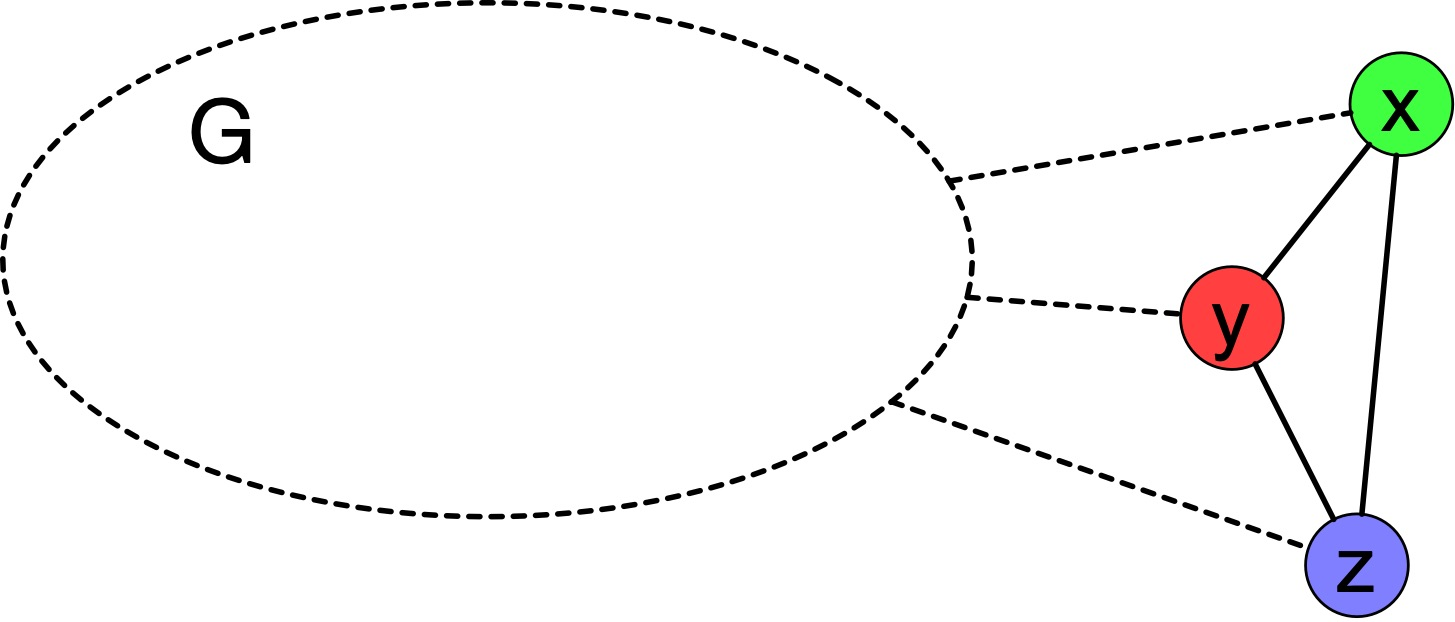
\includegraphics[width=0.45\textwidth]{img/6.jpg}
    \caption{Reduction from 4-COLORABILITY to 7-COLORABILITY}
    \label{ggg}
  \end{figure}

\item See Figure \ref{ggg}, suppose we have a function $f':V'\rightarrow \{1,2,3,4,5,6,7\}$ for the graph $G'$, then we have three different colors for $x,y,z$ (suppose the three colors are $1,2,3$). Since all vertices in $V$ are connected to $x,y,z$, they must have colors different from $1,2,3$, which must be $4,5,6,7$. Thus, we find $f:V\rightarrow \{4,5,6,7\}$ for $G$, and $G$ is 4-COLORABLE.

\end{itemize}

\newpage


\begin{exercise}
In the \textsf{MAX CUT} problem, we are given an undirected graph $G$ and an integer $K$ and have to decide whether there is a subset of vertices $S$ such that there are at least $K$ edges that have one endpoint in $S$ and one endpoint in $\bar{S}$. Prove that this problem is NP-complete.
\end{exercise}
\begin{proof}
    \leavevmode\newline
    \begin{itemize}
        \item Given a set of vertices $S$, we can get the number of edges that have one endpoint in $S$ and one endpoint in $\bar{S}$ in $O(E)$ time by traversing all edges in $G$, and compare the number to $K$. Thus the \textbf{max cut} problem is NP.
        \item 
    \end{itemize}
\end{proof}

\newpage


\begin{exercise}
Let \textsf{QUADEQ} be the language of all satisfiable sets of \textit{quadratic equations} over $0/1$ variables(a quadratic equations over $u_1,\ldots,u_n$ has the form $\sum_{i,j\in[n]}a_{i,j}u_iu_j=b$)where addition is modulo $2$. Show that \textsf{QUADEQ} is NP-complete.
\end{exercise}
\begin{proof}
    \leavevmode\newline
    \begin{itemize}
        \item 
    \end{itemize}
\end{proof}
\newpage


\begin{exercise}
In a typical auction of $n$ items, the auctioneer will sell the $i$th item to the person that gave it the highest bid. However, sometimes the items sold are related to one another(e.g., think of lots of land that may be adjacent to one another)and so people may be willing to pay a high price to get, say, the three items $\{2,5,17\}$, but only if they get all of them together. In this case, deciding what to sell to whom might not be an easy task. The \textsf{COMBINATORIAL AUCTION PROBLEM} is to decide, given numbers $n,k$, and a list of pairs $\{(S_i,x_i)\}^m_{i=1}$ where $S_i$ is a subset of $[n]$ and $x_i$ is an integer, whether there exist disjoint sets $S_{i_1},\ldots,S_{i_l}$ such that $\sum_{j=1}^lx_{i_j}\geq k$. That is, if $x_i$ is the amount a bidder is willing to pay for the set $S_i$, then the problem is to decide if the auctioneer can sell items and get a revenue of at least $k$, under the obvious condition that he can't sell the same item twice. Prove that \textsf{COMBINATORIAL AUCTION} is NP-complete.
\end{exercise}
\begin{proof}
    \leavevmode\newline
    \begin{itemize}
        \item 
    \end{itemize}
\end{proof}



\end{document}
